\chapter{Private Data in PDFs}

In \chapref{ch:introduction} we recounted a case in which the UK
Parliament inadvertently posted a PDF on a website containing
sensitive information about nuclear subs. But this is hardly a lone
incident. PDFs have been responsible for many kinds of privacy leaks
since the format was introduced by Adobe in 1983

\section{The PDF Format}

Adobe created PDF in the 1990s as a format that would allow computer
users to view and print electronic documents. PDF was designed as a
single electronic container that could be distributed, viewed, and
printed on practically any modern computer system without the need to
install  software or fonts other than a general purpose PDF
reader. Adobe released programs for making and reading PDFs,
originally called Acrobat Distiller and Acrobat Reader, but it also
published the format specification and licensed the patents required
to implement it. Today there are numerous programs that can create,
display and even edit PDF files, and the format has been adopted as an
international standard (ISO 32000-1:2008)\cite{ISO32000-1:2008}.

\subsection{Before PDF: PostScript}

Before PDF, electronic documents were typically distributed either as text
files, such as the Internet RFCs, or as PostScript
files. \emph{PostScript} is a programming language that Adobe Systems
created in the 1980s. The key idea 
of PostScript was that the language was interpreted by the printer, rather than 
the computer. This allowed relatively small amounts of data to be sent to
the printer, which would then render the page at the highest resolution
the device supported. But it also meant that the computer would be
freed from having to have drives for every different kind of printer
that might ever be on the market.

Listing~\ref{hello.ps} shows a simple PostScript program that draws a
black box and the words ``Hello World!''  The output of the program
(shrunk significantly) is shown at quarter size appears in
\figref{hello-ps-figure}. Even without reading a PostScript manual you
can draw some conclusions about the programming language simply by 
inspecting the listing and the resulting output:

\begin{itemize}
\item PostScript files begin with the magic number \verb|%!|.
\item Strings are enclosed in parentheses. 
\item Font names are preceded with slashes. 
\item Line drawing is performed with human-readable commands like
  ``moveto'' and ``drawto''. 
\item Arguments for commands come before the commands themselves,
  implying that PostScript is a stack-oriented language.
\end{itemize}

If you are interested, you can confirm most of these conclusions and
learn more about the language by reviewing an online PostScript tutorial.

\lstinputlisting[caption=A simple PostScript program]{ch-pdf/hello-ps.ps}\label{hello-ps-listing}

\begin{figure}
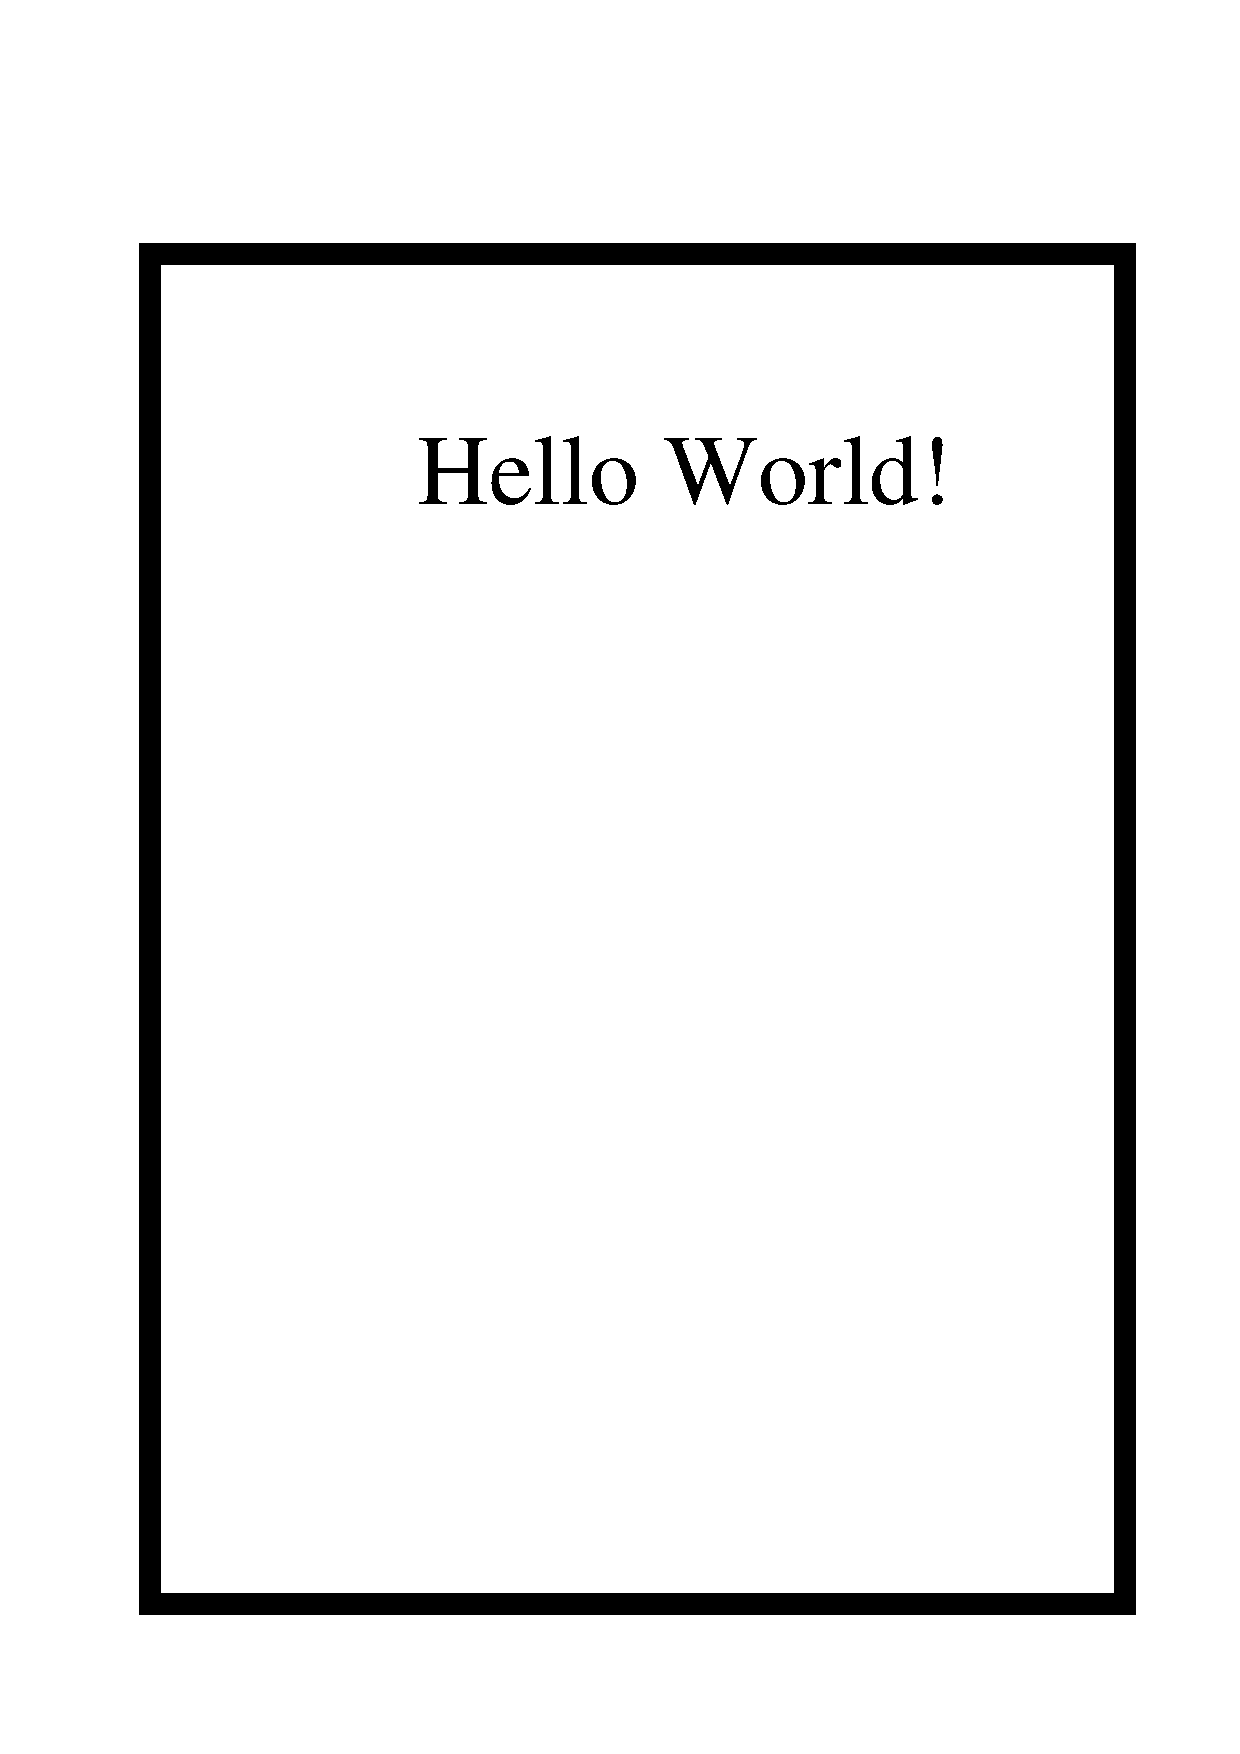
\includegraphics[scale=.25]{ch-pdf/hello-ps.pdf}
\caption{The output of Listing~\ref{hello-ps-listing}, shrunk to 25\% of
  the original size.}\label{hello-ps-figure}
\end{figure}


\subsection{The PDF Specification}

If you want to understand the internal PDF specification, you will have a much
easier time reading one of the earlier manuals than the later ones:

\begin{tabular}{lll}
Version & Year & Pages \\
\hline
PDF 1.2 & 1996 & 396 \\
PDF 1.3 (second edition) & 2000 & 696 \\
PDF 1.7 (part 1) & 2008 & 756\\
\end{tabular}




Unfortunately, PostScript's power made the language
less than ideal as a universal document format. First, the PostScript
is somewhat verbose, so PostScript files could get quite
large. Second, the PostScript execution context is not reset
after each page, so document pages can not be displayed out of
order: showing the contents of page 100 required first processing pages 1 through 99. PostScript also
lacks support for many features demanded in a modern electronic document format,
such as data encryption, digital rights management, and electronic forms.





PostScript's initial use was inside the Apple LaserWriter, the first
mass-market laser printer. There were inkjet printers, plotters, and
large-scale laser printers before the LaserWriter, but each 
had their own  language. With PostScript, application
programs didn't have to separately understand how to generate print
codes for each device. Instead, an
application program could simply generate PostScript and know that the
resulting page would be correctly printed. PostScript's most powerful features turned out to be
the ability to distribute high-quality line art as encapsulated
PostScript files that could embedded in other documents, scaled,
transformed, and then printed---all with little work on the part of
the application program. This, combined with the language's support
for high quality typography, made PostScript one of the key enabling
technologies of the 1980's boom in desktop publishing.


PDF was as an electronic page description language

Adobe introduced the PDF format in 1993. Since then, PDF has become an
international standard for distributing born-digital documents, scans
of paper documents, and even electronic forms~ 
PDF was designed as , and as
such it includes direct support for typography, line art and digital
photographs, as well as for document elements such as pagination,
bookmarks and metadata. 

PDF gained significant popularity in part because it could be used to 
distribute documents without the  risks of embedded viruses and
privacy-leaking metadata, and because PDF files could not be readily
modified after they were produced and distributed. But as PDF's popularity grew, additional
features were added to both the standard and Adobe's PDF Acrobat
reader. Today PDF can hold arbitrary files as attachments, PDF can
contain JavaScript programs, and PDF can hold significant amounts of
metadata. PDF files can also be edited with a wide variety of
programs, including the open source InkScape program.




In April 2011, the UK Parliament posted an
Adobe Acrobat Portable Document Format (PDF) file on its public website detailing key vulnerabilities of
UK nuclear subs. The electronic document had been cleared by the
British Ministry of Defense, where an official had been charged with
removing the sensitive portions, but the redactions were made incorrectly: the sensitive text had
simply been obscured with a black box, and could be
recovered by  copying the text out of the PDF file and pasting
it into a word processor. The
result was a document that appeared to  be properly redacted, but
which still contained state secrets.  A follow-up investigation by
\emph{The Daily Telegraph} found similar  PDF files on other UK government websites
found four other documents where sensitive
information was improperly ``redacted''\cite{telegraph-april2011-secrets}.

Leaks of sensitive information  in PDF files are frequently
newsworthy, but they are hardly new. In October 2003, the US Justice
Department posted a report on its website about the Department's
internal efforts at increasing racial diversity---but every conclusion and
recommendation was blacked out. The
redaction was imperfect: journalist
Russ Kick discovered that the black boxes
could be easily removed~\cite{nyt-diversity-critical}. 

``PDF'' is the Portable Document Format, developed by Adobe in the
1990s as a universal file format for describing printed documents. 

\section{Improperly redacted data}
\section{High-resolution JPEGs}
\section{High-resolution line drawing}
medical information leakage.
\section{Metadata}
\section{References}

\bibentry{nsa-pdfs}


